\subsubsection{Trivsel vs åpenhet}

Gruppen har alltid kommunisert på en inkluderende og høflig måte. 
Særlig i starten er det vanlig at samtaler er preget av forsiktig og overfladisk innhold. 
For at kommunikasjonen i en gruppe skal være svært direkte og åpen, kreves det oftest at medlemmene føler seg komfortable og kjent med resten av gruppen. 
En slik utvikling ble antydet i flere samarbeidsindikatorer. 
Samarbeidsindikatoren baseres på en spørreundersøkelse som holdes tidlig, midtveis og sent i semesteret. \\

Hovedfokuset for samarbeidsindikatoren har vært å følge utviklingen av det sosiale samværet, samt diskutere hvilke effekter dette har hatt på gruppens produktive kapasitet. Resultatet av undersøkelsen ble fremstilt i et diagram med fire akser: \textit{Ærlig og direkte}, \textit{forpliktet og tillitsfull}, \textit{effektiv og strukturert} og \textit{åpen og lyttende}. Jo lengre vekk fra sentrum, jo bedre. I forbindelse med kommunikasjon i gruppen, er punktet som kalles \textit{Ærlig og direkte} den viktigste. Uten ærlig og direkte kommunikasjon kan et gruppesamarbeid resultere i at ikke-tema (\textit{'Alle vet det' - ingen snakker om det} oppstår. Indikatorene er gitt i figur \ref{samind1}, \ref{samind2} og \ref{samind3}.

\begin{figure}[h!]
  \caption{Samarbeidsindikator 1 basert på undersøkelse landsbydag 5.}
  \centering
    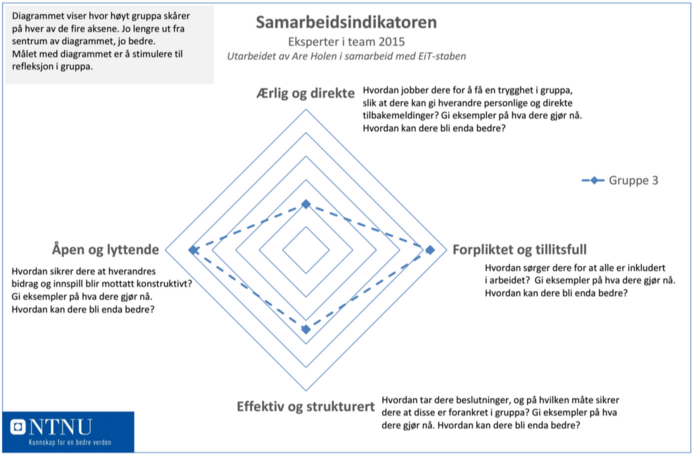
\includegraphics[width=0.5\textwidth]{Bilder/samarbeidsindikator1.png}
    \label{samind1}
\end{figure}

\begin{figure}[h!]
  \caption{Samarbeidsindikator 2 basert på undersøkelse landsbydag 9.}
  \centering
    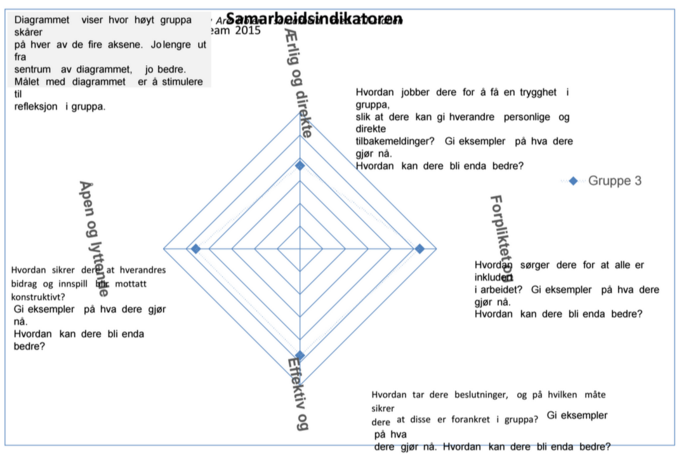
\includegraphics[width=0.5\textwidth]{Bilder/samarbeidsindikator_2.png}
    \label{samind2}
\end{figure}

\begin{figure}[h!]
  \centering
    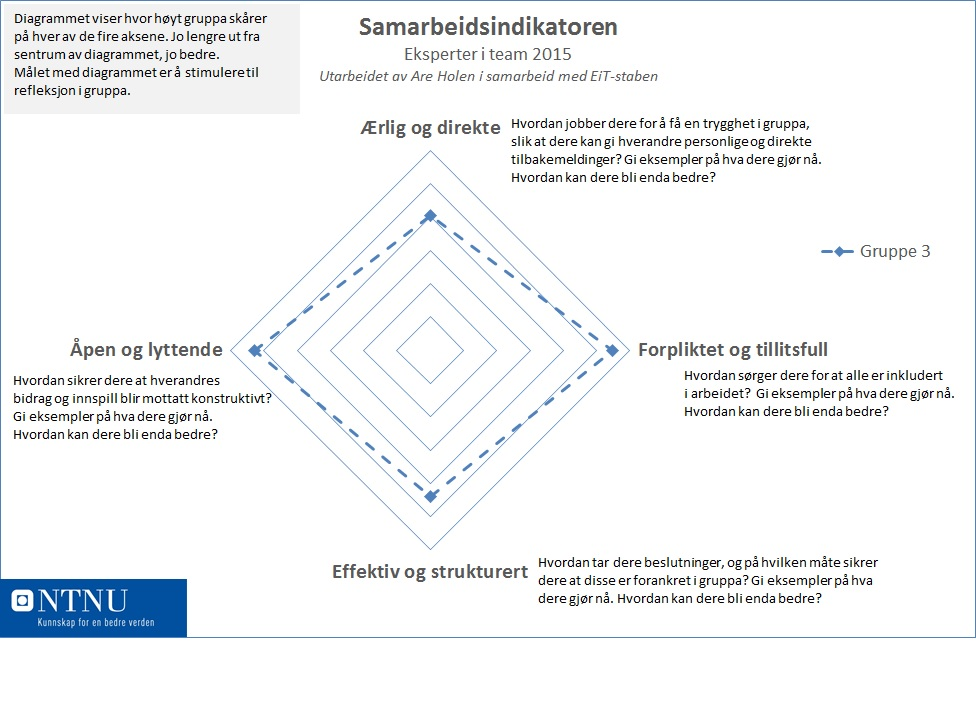
\includegraphics[width=0.5\textwidth]{Bilder/samarbeidsindikator_3.jpg}
    \caption{Samarbeidsindikator 3 basert på undersøkelse landsbydag 14.}
    \label{samind3}
\end{figure}

Den første samarbeidsindikatoren, figur \ref{samind1} antyder at gruppen ikke har vært klart ærlig og direkte.
En naturlig årsak til at gruppen scoret lavt på ærlig og direkte, kan være at medlemmene ikke ønsket å ødelegge den positive stemningen. Gruppen hadde samarbeidet i så kort tid at mottagelsen av direkte tilbakemeldinger og kritikk, fortsatt var ukjent. Resultatet var ikke en stor overraskelse for gruppen, da få situasjoner som inneholdt kritikk av noe slag hadde oppstått. Det ble enighet om at årsaken ikke var at gruppen og medlemmene ikke ville håndtere kritikk på en konstruktiv måte, men at utfallet var en naturlig følge av at samarbeidet var i en tidlig fase. Indikatoren stimulerte til at det å gi ærlig og direkte tilbakemelding, ble satt i fokus. \\

Gjennomgående for alle samarbeidsindikatorene var at gruppen scoret dårligst på vurderingskriteriet \textit{ærlig og direkte}. 
Utviklingen har likevel vært positiv, da de neste to indikatorene, figur \ref{samind2} og \ref{samind3}, viser forbedring (punktet har beveget seg vekk fra sentrum). 
Et konkret eksempel på å gi og få tilbakemelding fra medlemmene, var under grupperefleksjonen på slutten av dagen da de to som hadde hatt rolle som ordstyrer og referent, fikk direkte tilbakemelding. Under refleksjonen landsbydag 6 sa Martin: \textit{"Simen mangler litt autoritet som ordstyrer. Kanskje han er for snill. Han kunne vært tydeligere på hvordan ting skulle blitt gjort, som for eksempel å innlede en 'runde rundt bordet'."}. Slik tilbakemelding ga positive konsekvenser både for gruppen og for medlemmet som mottok den. Neste gang Simen var ordstyrer var det tydelig at han hadde tatt kritikken til seg, og lært fra forrige gang.
Ved å gi tilbakemelding på en så konkret oppgave som ordstyrerrollen, ble terskelen også lavere ved andre situasjoner. \\

Som nevnt i starten, har gruppen alltid kommunisert på en høflig og positiv måte. I starten skyldtes høfligheten at medlemmene kun kjente hverandre på en overfladisk måte, og at kommunikasjonen ble preget av dette. I slutten av samarbeidet var kommunikasjonen fortsatt like positiv, men på helt annet grunnlag. Medlemmene kunne gi positive og konkrete tilbakemeldinger på hverandres arbeid basert på at hver enkelts sterke sider hadde blitt avdekket. 






















<<<<<<< HEAD


=======
Analysere sosiogram + sosiale inntrykk Anna
\\
Andre kommunikasjonstrender som har blitt observert i gruppen er en økt grad av frie samtaler, småprat og humor. Spesielt Martin og Karsten har hatt lett for å skape digresjoner, slik at resten av gruppen har måttet be dem om å beholde fokus. 
Kommunikasjonsmønsteret i gruppen har under hele prosessen endret seg.
Noen ganger gradvis og sakte, andre ganger raskere. 
\\
>>>>>>> origin/master
